L'implémentation est un processus qui nécessite une approche méthodique, combinant recherche, développement et tests. Dans le cadre de ce projet, cette phase a été cruciale pour garantir la réussite de la génération et de la manipulation des fichiers d'entrée du modèle CROCO.

Mon parcours d'implémentation a débuté par une phase intensive de recherche et d'acquisition d'informations. Le site officiel de CROCO(\cite{crocoofficial}) a été une ressource inestimable, fournissant des détails techniques et des orientations sur les fichiers d'entrée. De plus, le CROCO-Tool(\cite{crocotool2007}), avec sa riche documentation et ses exemples, a été un guide essentiel pour comprendre les nuances des données nécessaires.

Avec ces connaissances en main, j'ai entamé la phase de développement en écrivant des scripts en Python. Ces scripts étaient destinés à automatiser et à faciliter la génération des fichiers d'entrée, en s'assurant qu'ils étaient conformes aux exigences du modèle CROCO.

Suite à cette étape, j'ai commencé à explorer l'API de QGIS. L'objectif était d'intégrer mes scripts Python directement dans le plugin QCrocoflow. Cette intégration permettrait non seulement d'automatiser la génération des fichiers d'entrée directement depuis QGIS, mais aussi de fournir une interface utilisateur intuitive pour les utilisateurs du plugin. L'utilisation de l'API de QGIS a ouvert la porte à une interaction plus fluide entre les données géospatiales et le modèle CROCO, rendant le processus de simulation plus transparent et efficace.

\subsection{Guides}

%\begin{figure}[H]
	%\centering
	%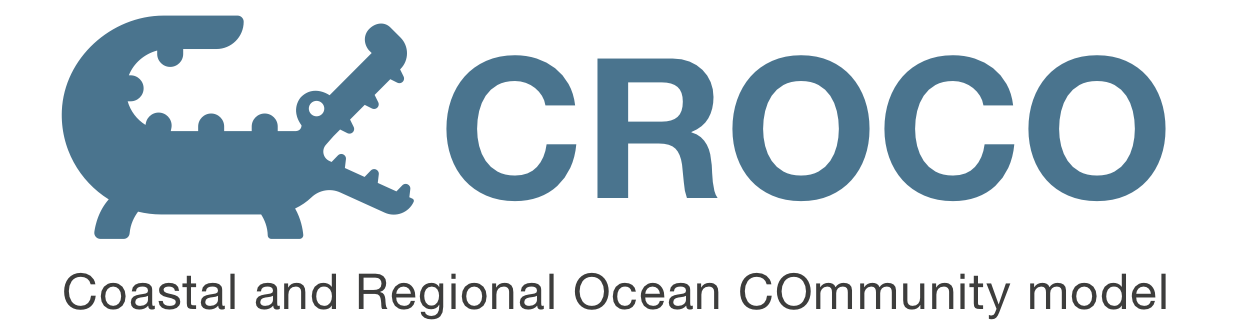
\includegraphics[height=1in]{./IMAGES/croco.png}
	%\caption[LOGO CROCO]{croco logo}
	%\label{fig:croco}
%\end{figure}



\subsubsection{Grid}
todo
\subsubsection{Tides}
todo
\subsubsection{BULK}
todo